%!TEX root = ../thesis.tex
The original basis for this thesis was born from a fascination of things that \emph{moves, adapts and changes} - the bringing of ``life'' to the objects and environments that surrounds us, letting them transform to our needs, both in function and form. 

The fascination of giving life to inanimate objects is not entirely new.
A famous example of this is the Vaucanson Duck, an automata created by the French inventor and artist Jacques Vaucanson in 1739 \citep{riskin2003defecating}.
It was later depicted by a nineteenth-century inventor, as seen in figure~\ref{vaucanson_duck} 
The mechanical duck, which supposedly contained over a thousand parts, could both flap its wings and appeared to have the ability to eat, digest, and defecate grains.

The animation of `things' still amazes today, both in the world of technology, with advancements in robotics, and in the world of crafts where ingenuity and craftsmanship can give rise to fascination.   
An example of the latter is Theo Jansen's that gives life to new species of animals with his amazing Strandbeests \cite{strandbeestJansen}.  
Made mostly from yellow plastic tube and fabric sails, these skeletons traverses the beaches of the Netherlands, living off the wind, adapting to the turnings of the elements, see figure~\ref{strandbeest}.

\begin{figure}[h]
	\centering
	\begin{minipage}{.45\textwidth}
		\centering
		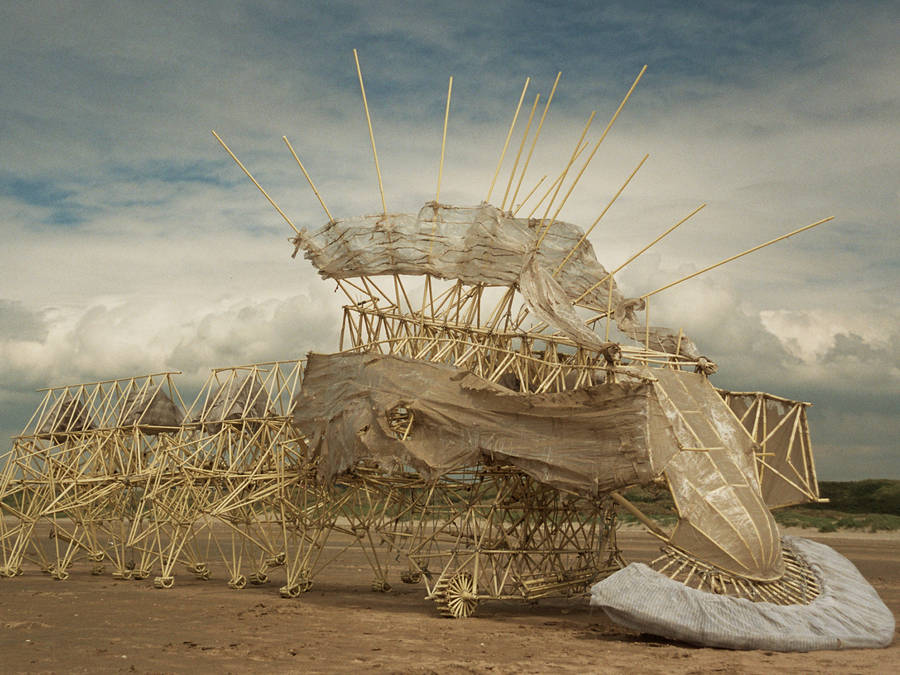
\includegraphics[width=0.9\linewidth]{figures/strandbeest}
		 \captionof{figure}{One of Jansen's Strandbeests, \citep{strandbeestJansen}}
		\label{strandbeest}
	\end{minipage}%
	\hspace{0.1cm}
	\begin{minipage}{.45\textwidth}
		\centering
		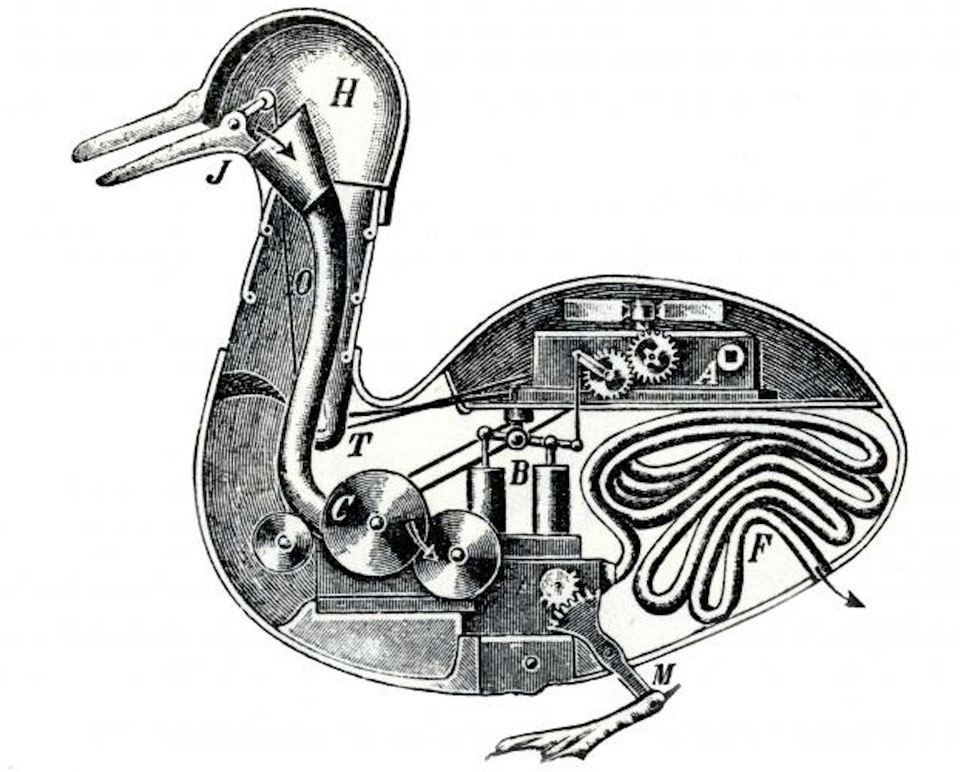
\includegraphics[width=0.9\linewidth]{figures/vaucanson_duck}
		\captionof{figure}{A nineteenth-century inventor's imagined depiction of the inner workings of the Vaucanson Duck \citep{riskin2003defecating}}
		\label{vaucanson_duck}
	\end{minipage}	
\end{figure}

These two examples, each impressive in their own right, points to the powerful expressiveness that actuation can give objects, as we have a tendency to relate things that move to living entities. 
\blank
In this chapter we will attempt to bring together some of the ideas that has laid the ground and motivation for our thesis work.
Our process has not been on an entirely straight line, so at the same time we will try to draw lines between the different areas and disciplines that have shaped and influenced our process and ideas into the end result we present in this thesis.  
\blank
Her er skal der skrives om tingene fra noterne
\blank
\todo{afrunding herfra, udkast}

In the midst of all these seemingly divergent digressions we believe that there is an unexplored space for interfaces that focuses on adaptability and situational awareness, that function on the terms of the user and not the computer system, bringing a more dynamic relationship, as seen in software, into the world of physical interactable artefacts.  

Noter:
\begin{verbatim}
Hvad er status nu og her og hvad er mulighederne
- ``men, der er faktisk et rum som ikke er udforsket'' - det tidslige, situerede

Computerfokus vs brugerfokus
- Contextual interfaces vs Ad hoc interfaces
- Hvordan kan man give brugeren kontrollen tilbage (i modsaetning til CA)
- Refererende perspektiv - Participatory design - demokratisere - empower the user
- Eksempelvis: end-user-programming
- Tilgangen peger paa et design rum

Hjemmet
- Hvad er et hjem
- Vi fokuserer paa hjemme - en valgt begraensning/omraade med potentiale
- S. Brand og struktur
- Hvad hjemmet betyder for dem der bor der

DIY og infrastruktur
- Balance mellem producent og bruger
- Traditionelle crafts (fra Coelho)

Digital vs fysisk
- Materialitet (shapechange, digital bits)


Afslutte med en aabning til projektet - hvordan vi med udgangspunkt i ovenstaaende har bevaeget os videre, hvad vil vi udforske.
\end{verbatim}